\chapter{Magnetismo de sólidos} \label{Ch:10}

En este Capítulo se estudian algunas de las contribuciones más importantes al magnetismo de los sólidos. Como se verá, alguna de ellas (como la ferromagnética) constituye un fenómeno cooperativo que lleva asociado una transición de fase. Es también destacable que el magnetismo de sólidos es en buena medida un efecto cuántico dado que muchas de sus causas (el momento mangnético de espín, la interacción de intercambio, etc.) no tienen análogo clásico.

\section{Relaciones básicas}


\section{Diamagnetismo atómico}

\section{Paramagnetismo atómico}

\subsection{Origen del momento mangnético atómico}

\subsection[Dependencia de la magnetización respecto $\vec{\Bn}$ y $T$]{Dependencia de la magneteización paramagnética con la temperatura y el campo magnético}

\subsection{Ley de Curie}

\section{Paramagnetismo de los electrones de conducción}

\section{La interacción de intercambio}

\section{Ferromagnetismo}

\section{Dominios ferromagnéticos}

\section{Orden ferrimangnético}

\begin{figure}[h!] \centering
	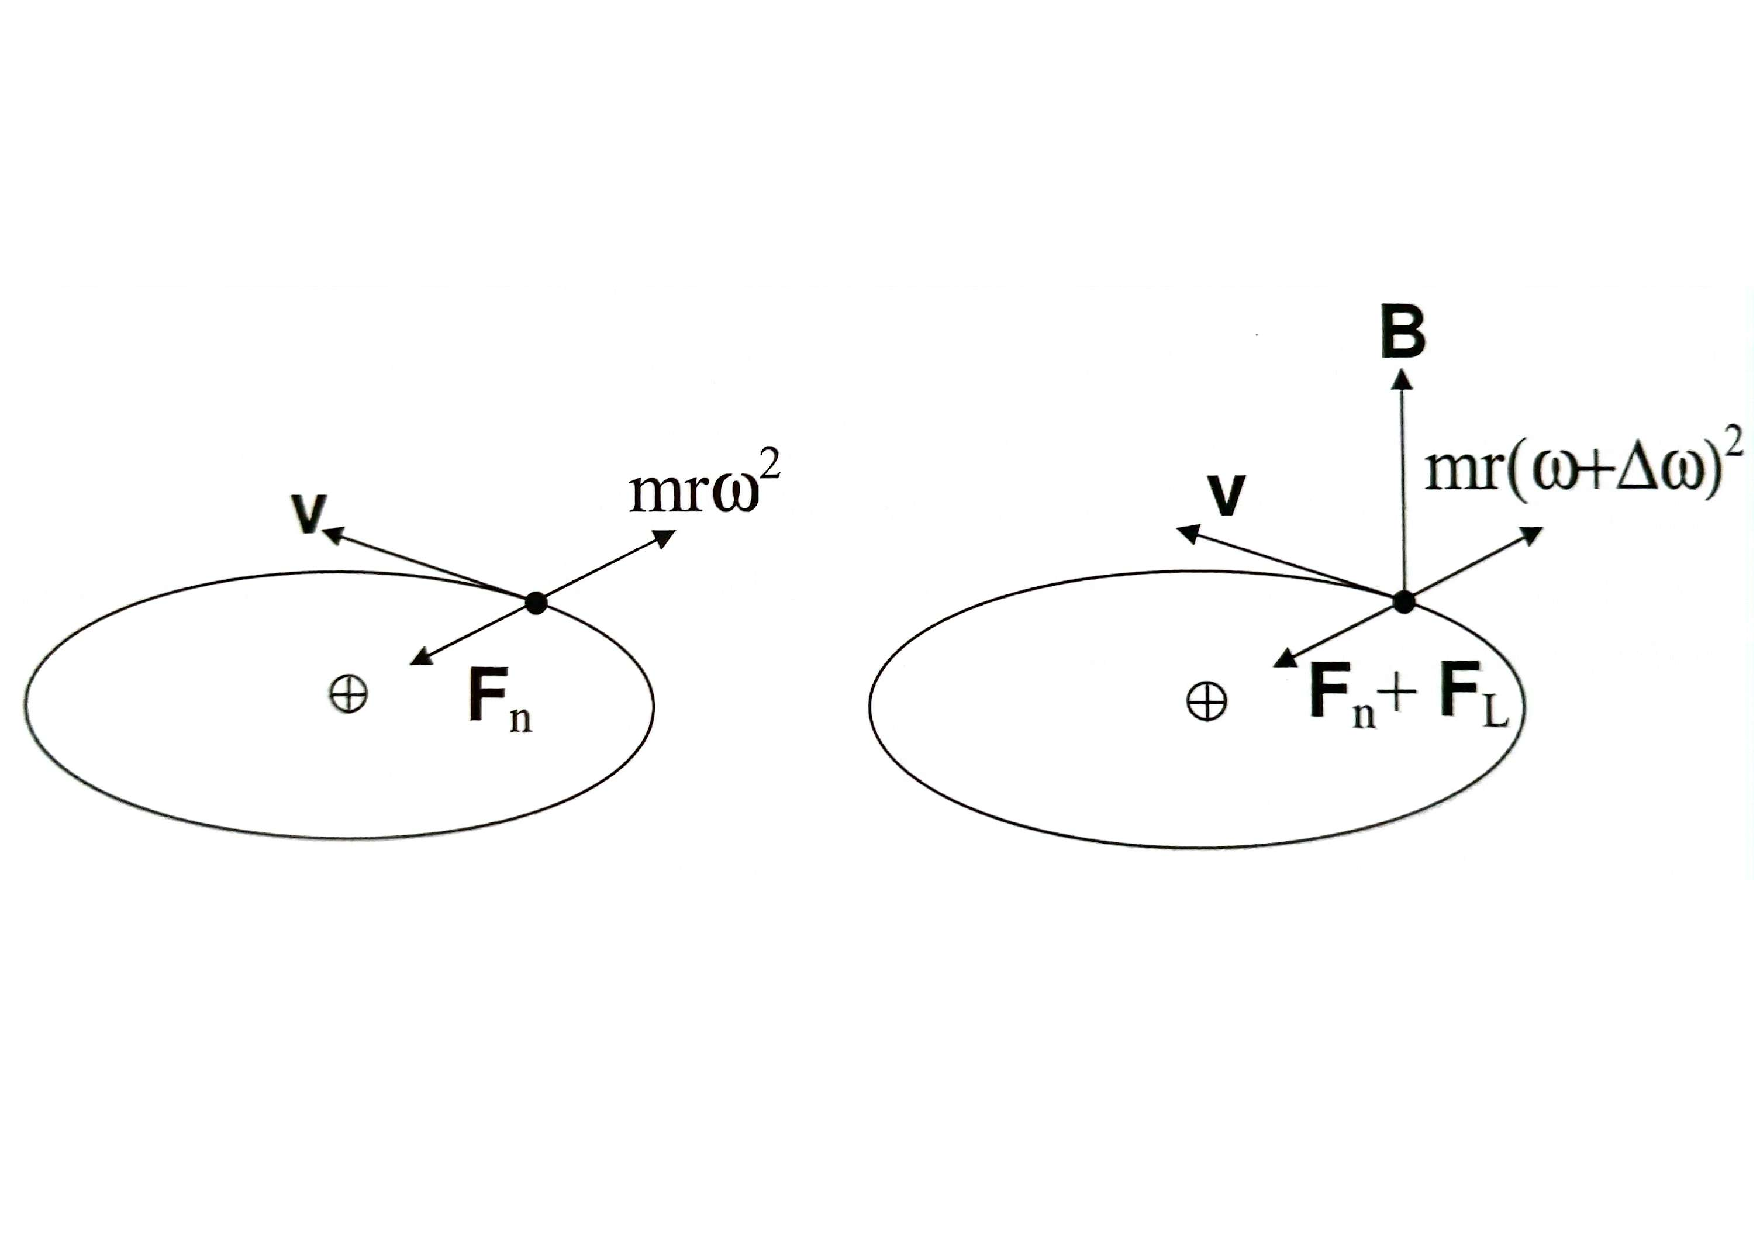
\includegraphics[scale=0.35]{Cuerpo/Ch_10/Fotos libro 1.pdf}
	\caption{Balance  de fuerzassobre un electrón orbitando en torno a un núcleo en ausencia (izquierda) o en presencia (derecha) de un campo mangético externo. El referencial usado es uno centrado en el núcleo y que gira con el electrón de modo qeu hay que considerar las fuerzas inerciales (aquí sólo hay fuerza centrífuga).}
	\label{Fig:10-01}
\end{figure}
\begin{figure}[h!] \centering
	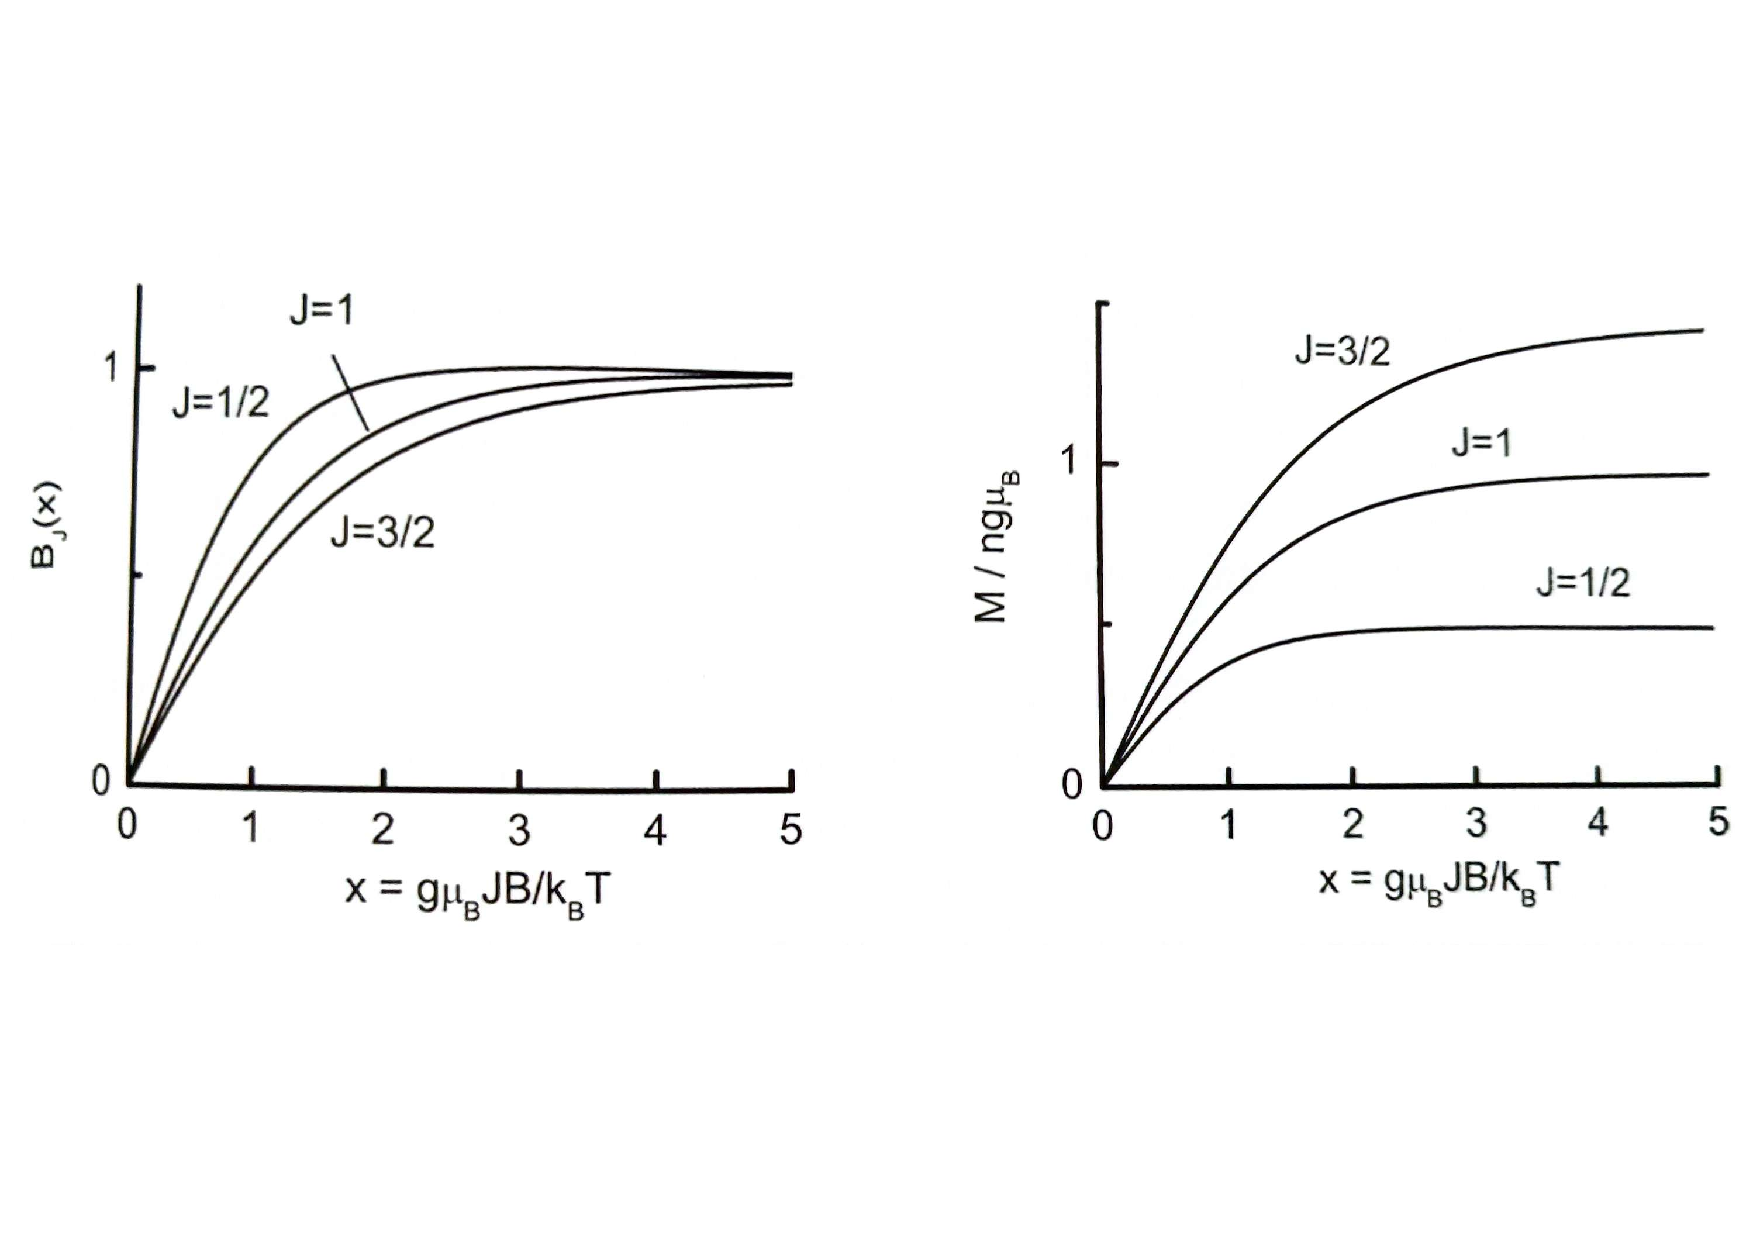
\includegraphics[scale=0.35]{Cuerpo/Ch_10/Fotos libro 2.pdf}
	\caption{Dependencia con $x$ de la función de Brillouin y de la magnetización paramagnética para distintos valores de $J$.}
	\label{Fig:10-02}
\end{figure}
\begin{figure}[h!] \centering
	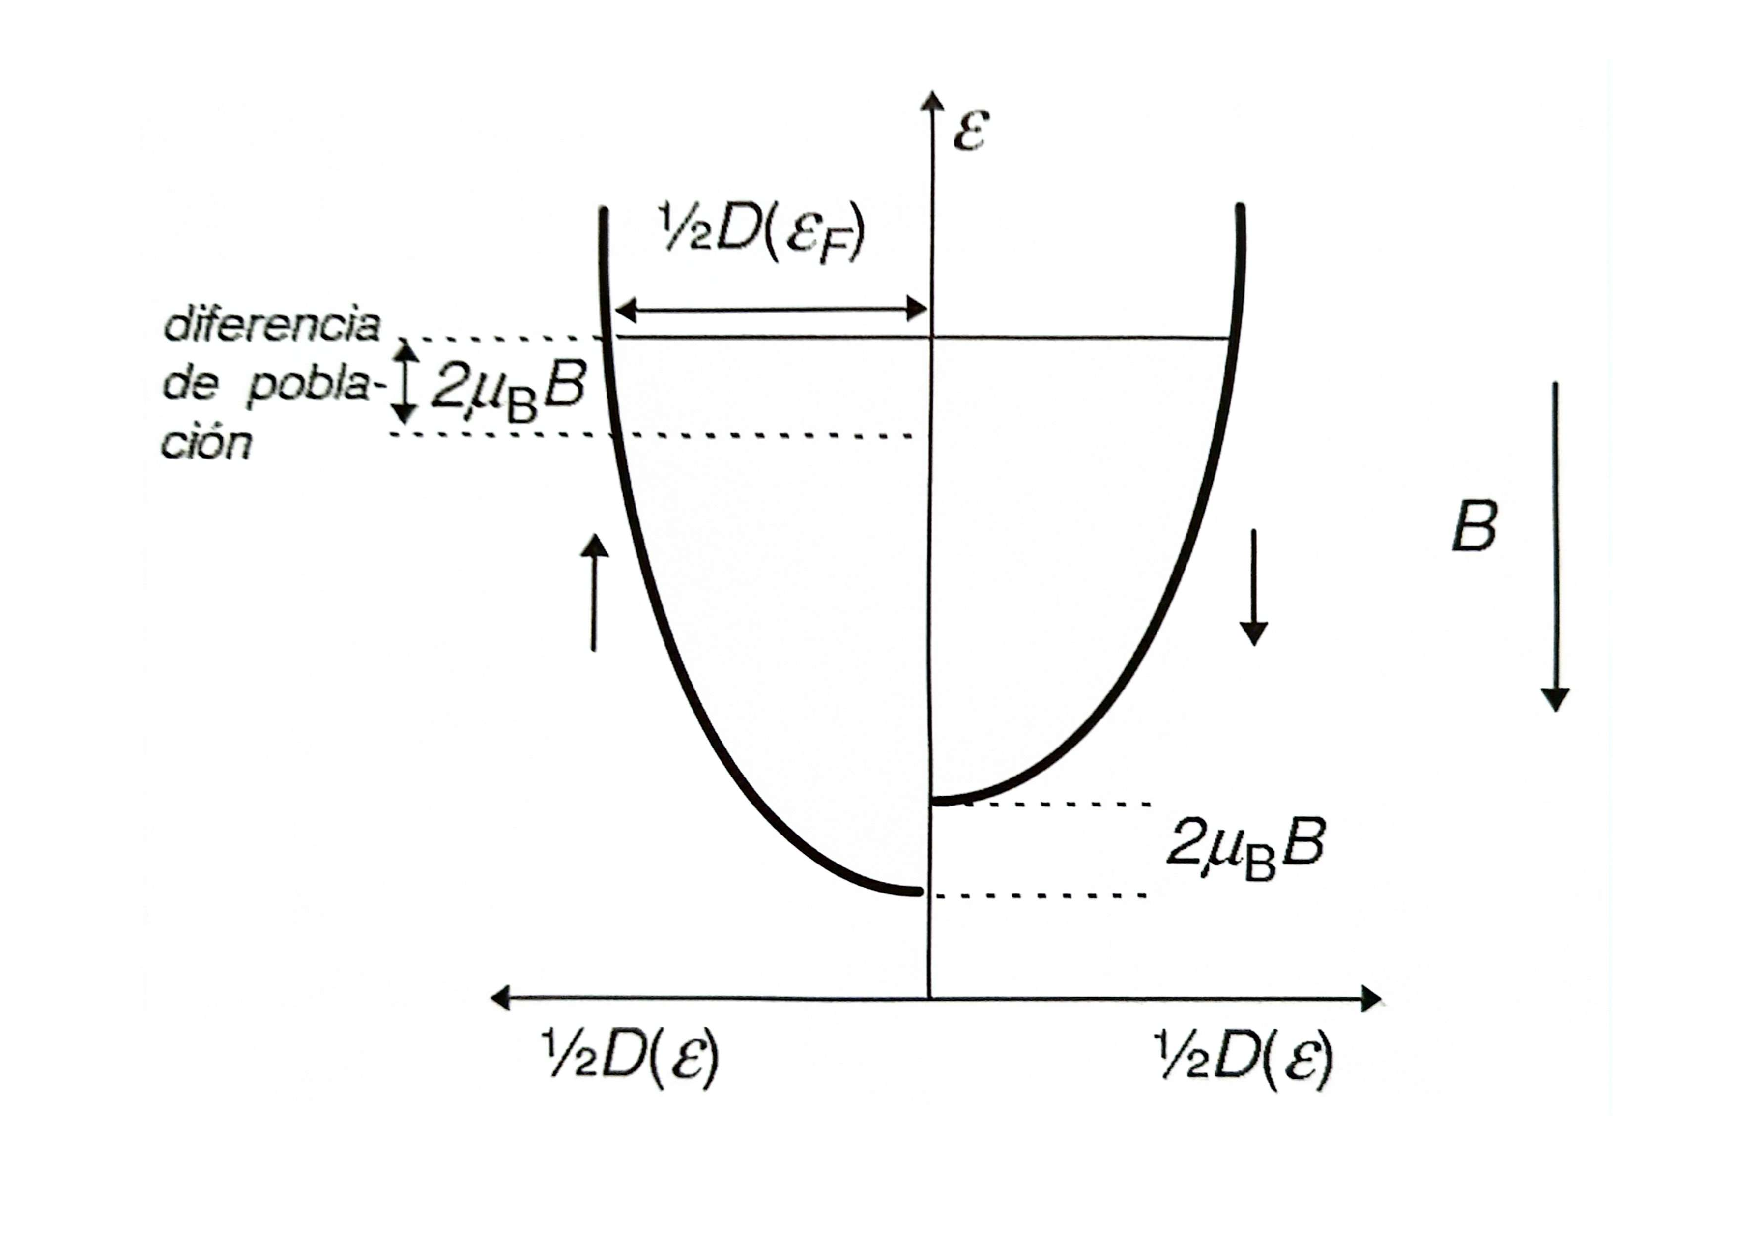
\includegraphics[scale=0.35]{Cuerpo/Ch_10/Fotos libro 3.pdf}
	\caption{Desplazamiento relativo de los niveles energéticos electrónicos correspondientes a espín $\uparrow$ y espín $\downarrow$.}
	\label{Fig:10-03}
\end{figure}
\begin{figure}[h!] \centering
	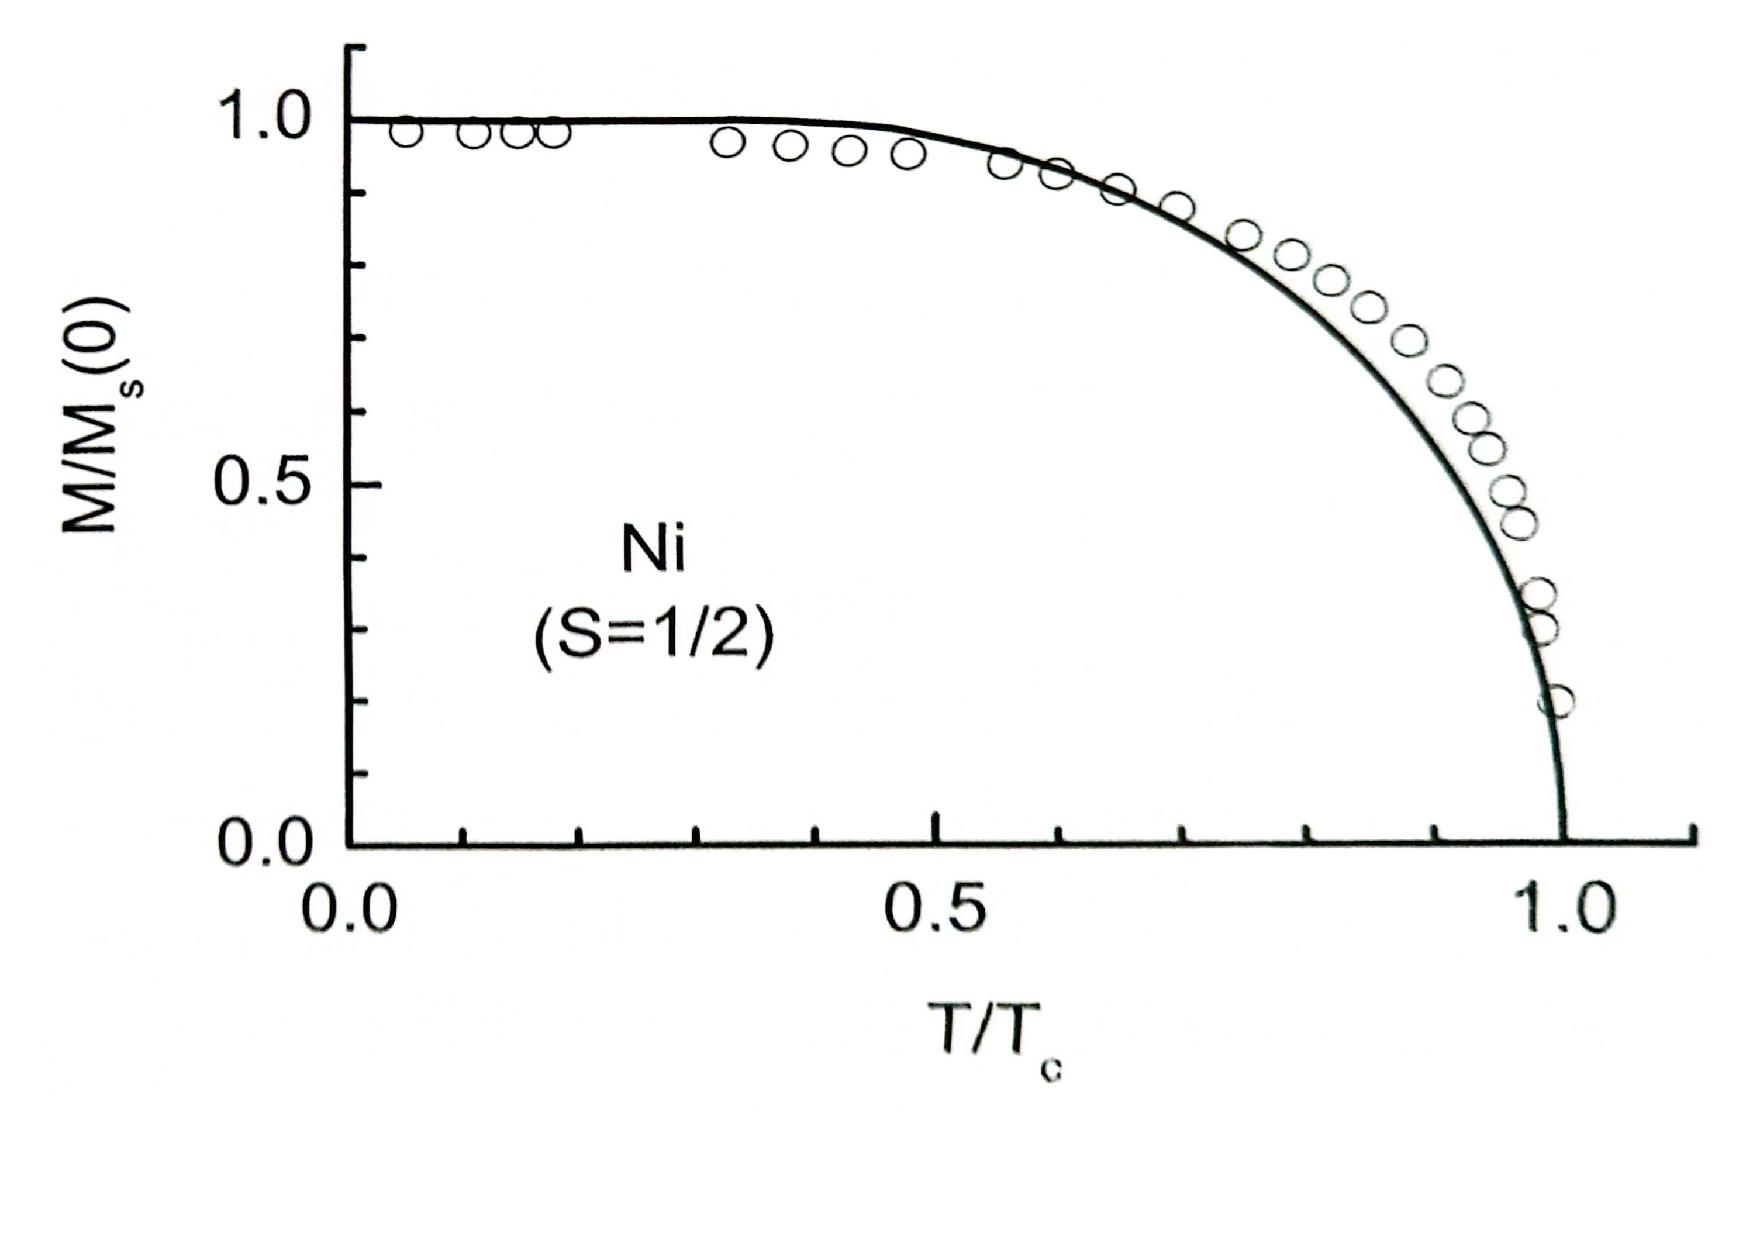
\includegraphics[scale=0.35]{Cuerpo/Ch_10/Fotos libro 4.pdf}
	\caption{Dependencia con la temperatura de la magnetización espontánea para el Ni cuando $T<T_C$, y compensación con las predicciones de campo medio.}
	\label{Fig:10-04}
\end{figure}
\begin{figure}[h!] \centering
	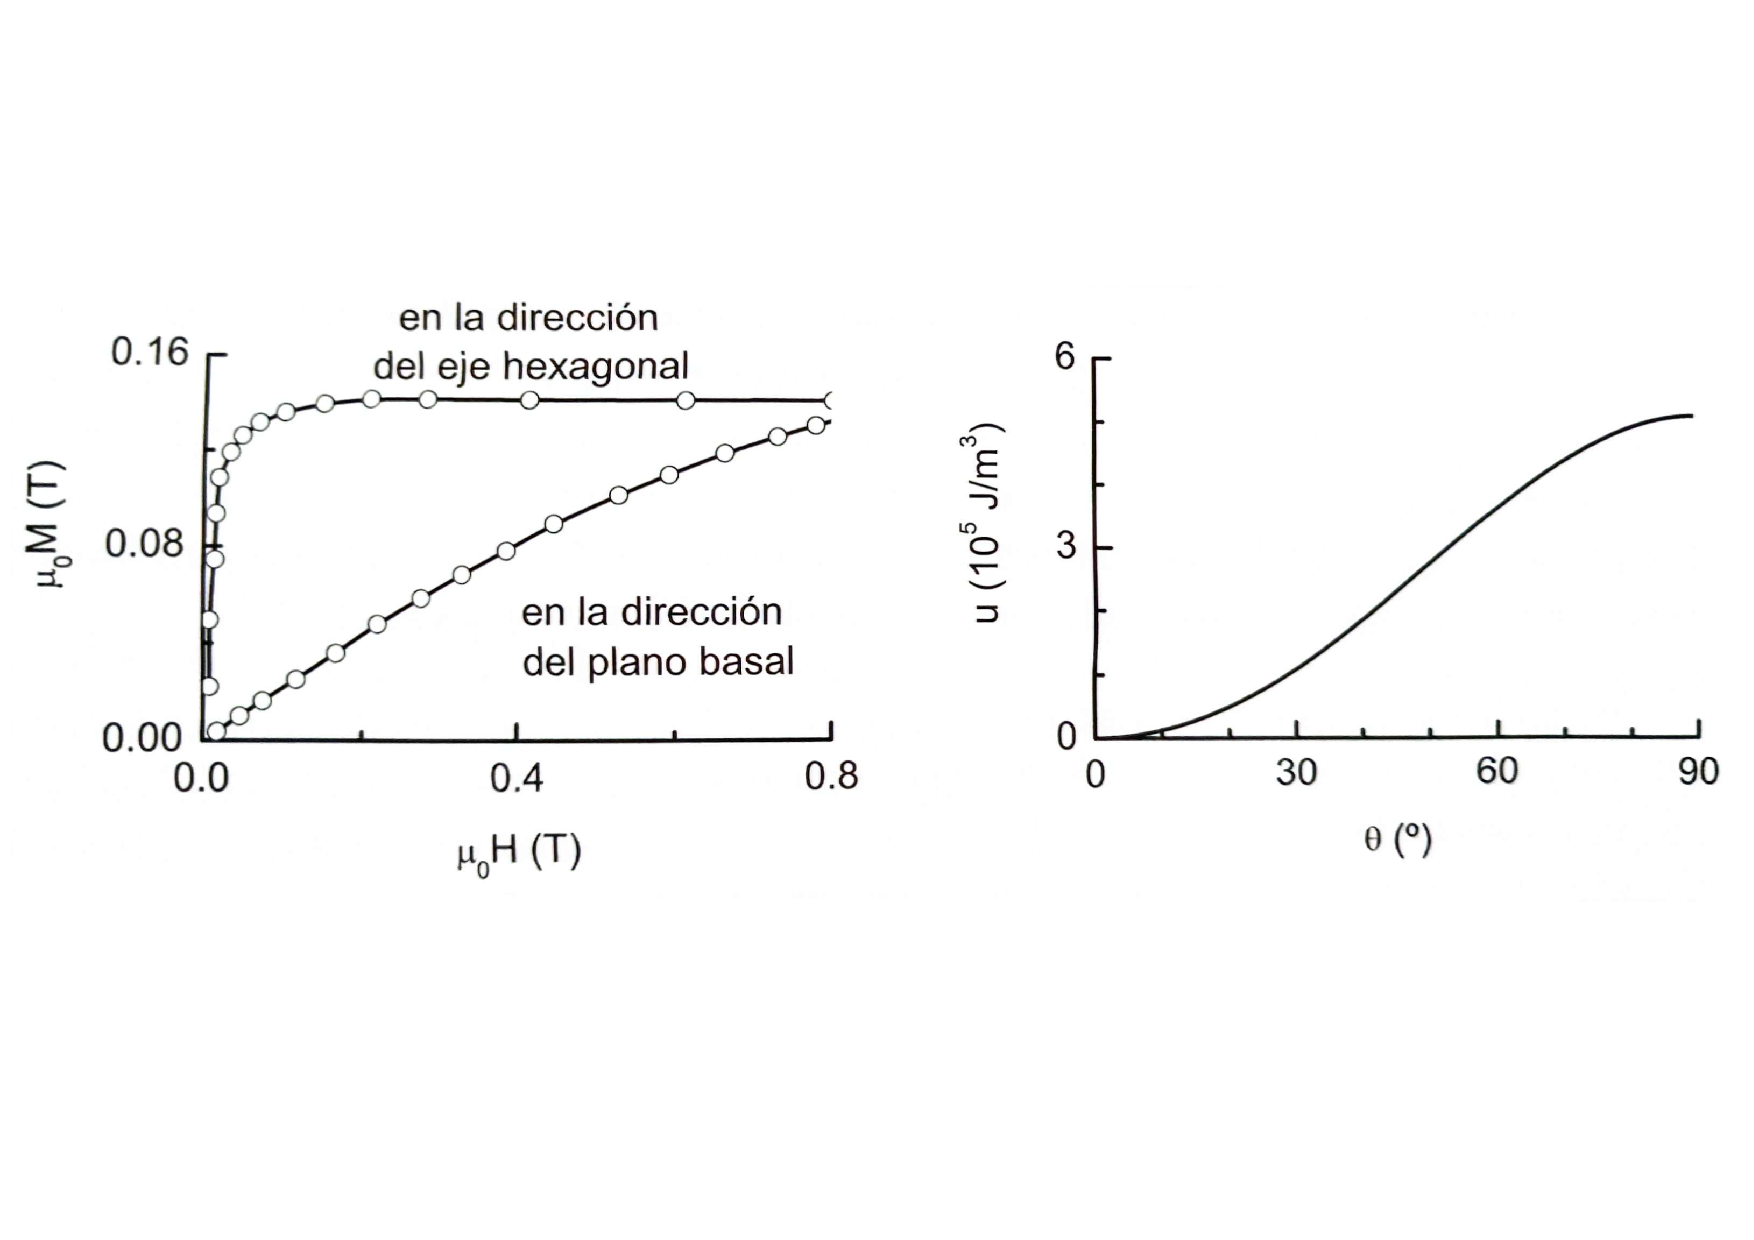
\includegraphics[scale=0.35]{Cuerpo/Ch_10/Fotos libro 5.pdf}
	\caption{En la izquierda la magnetización de una muestra de  Co para las direcciones paralela y perpendicular al plano basal de la estructura hexagonal. En la derecha de anisotropía del Co según el ángulo que forma la magnetización con el eje hexagonal.}
	\label{Fig:10-05}
\end{figure}
\begin{figure}[h!] \centering
	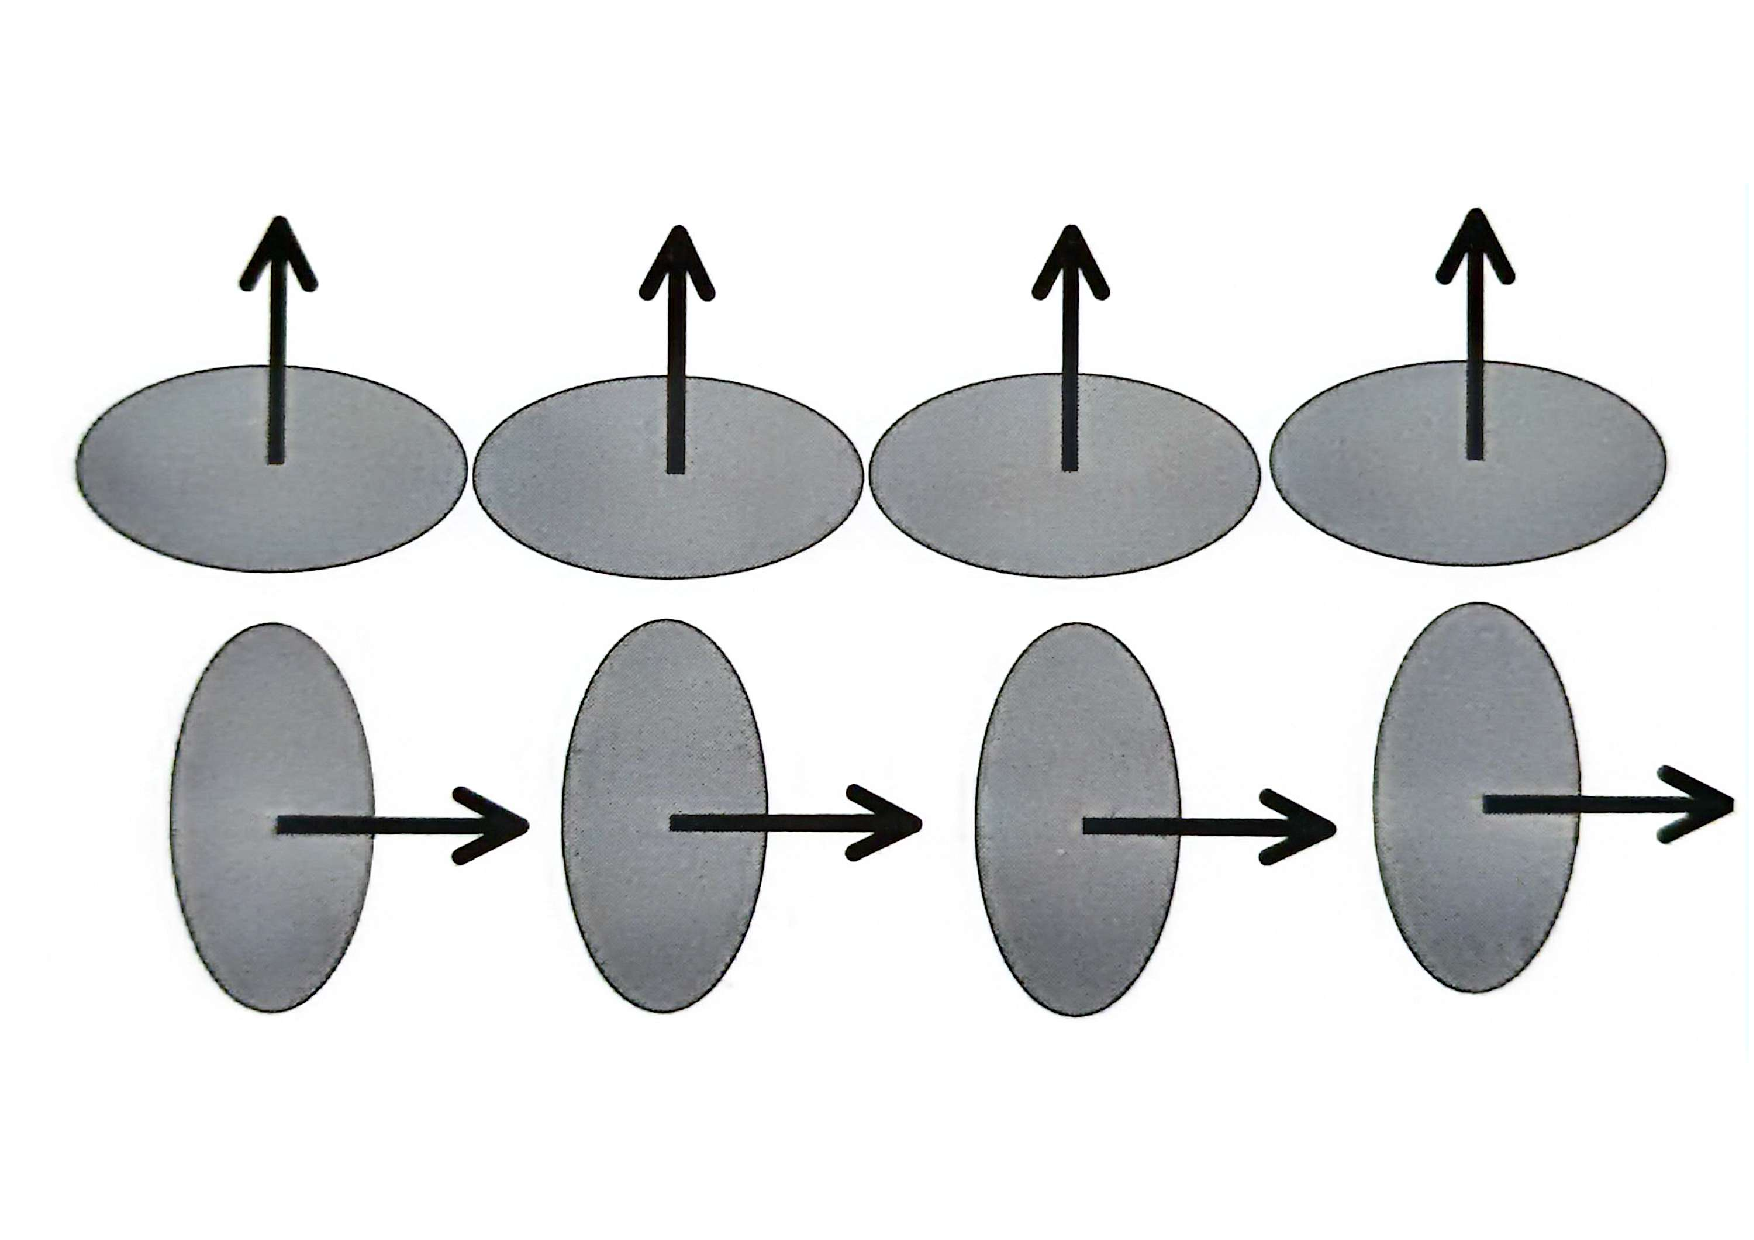
\includegraphics[scale=0.35]{Cuerpo/Ch_10/Fotos libro 6.pdf}
	\caption{Distribución electrónica para diferntes orientaciones del campo mangético aplicado.}
	\label{Fig:10-06}
\end{figure}
\begin{figure}[h!] \centering
	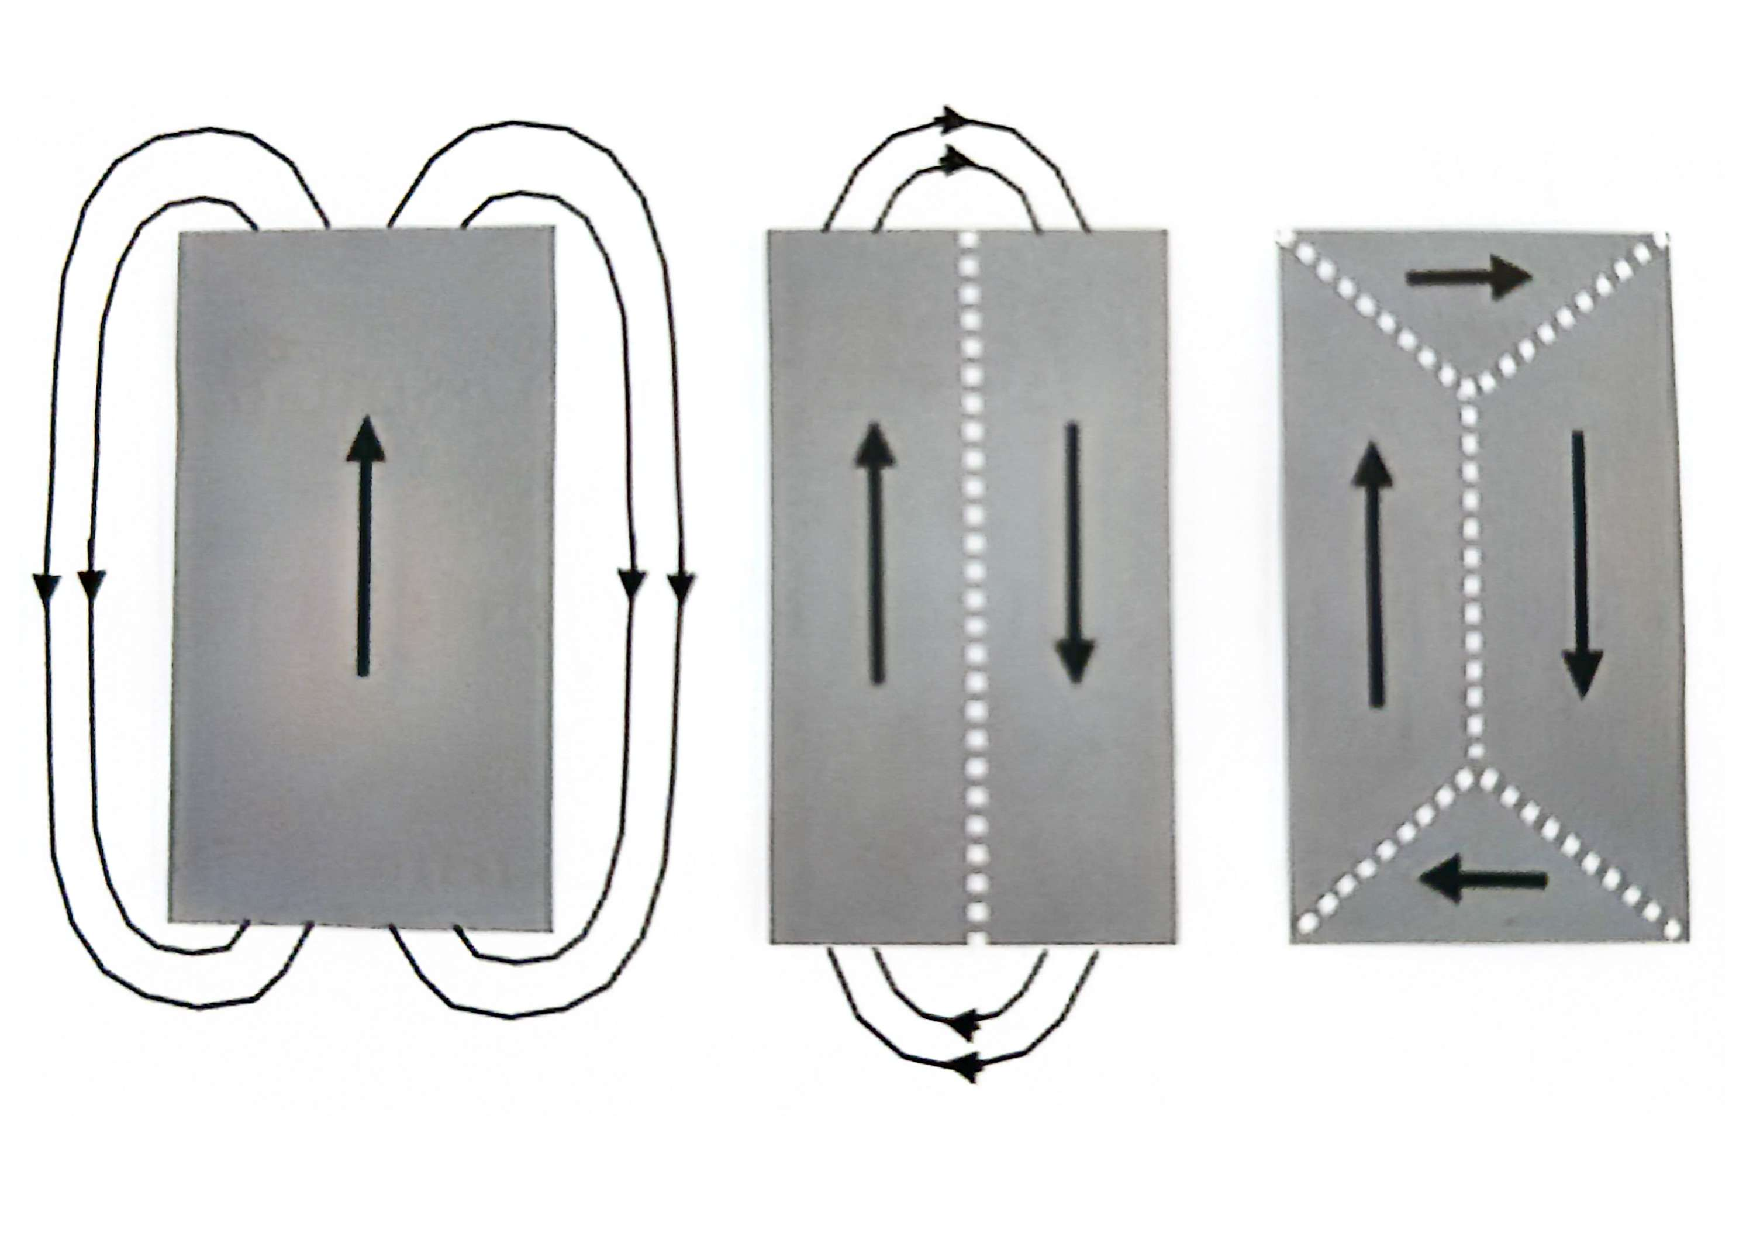
\includegraphics[scale=0.35]{Cuerpo/Ch_10/Fotos libro 7.pdf}
	\caption{Aparición de dominios en una muestra ferromagnética. Las flechas indican la orientación de los momentos magnéticos en cada dominio.}
	\label{Fig:10-07}
\end{figure}
\begin{figure}[h!] \centering
	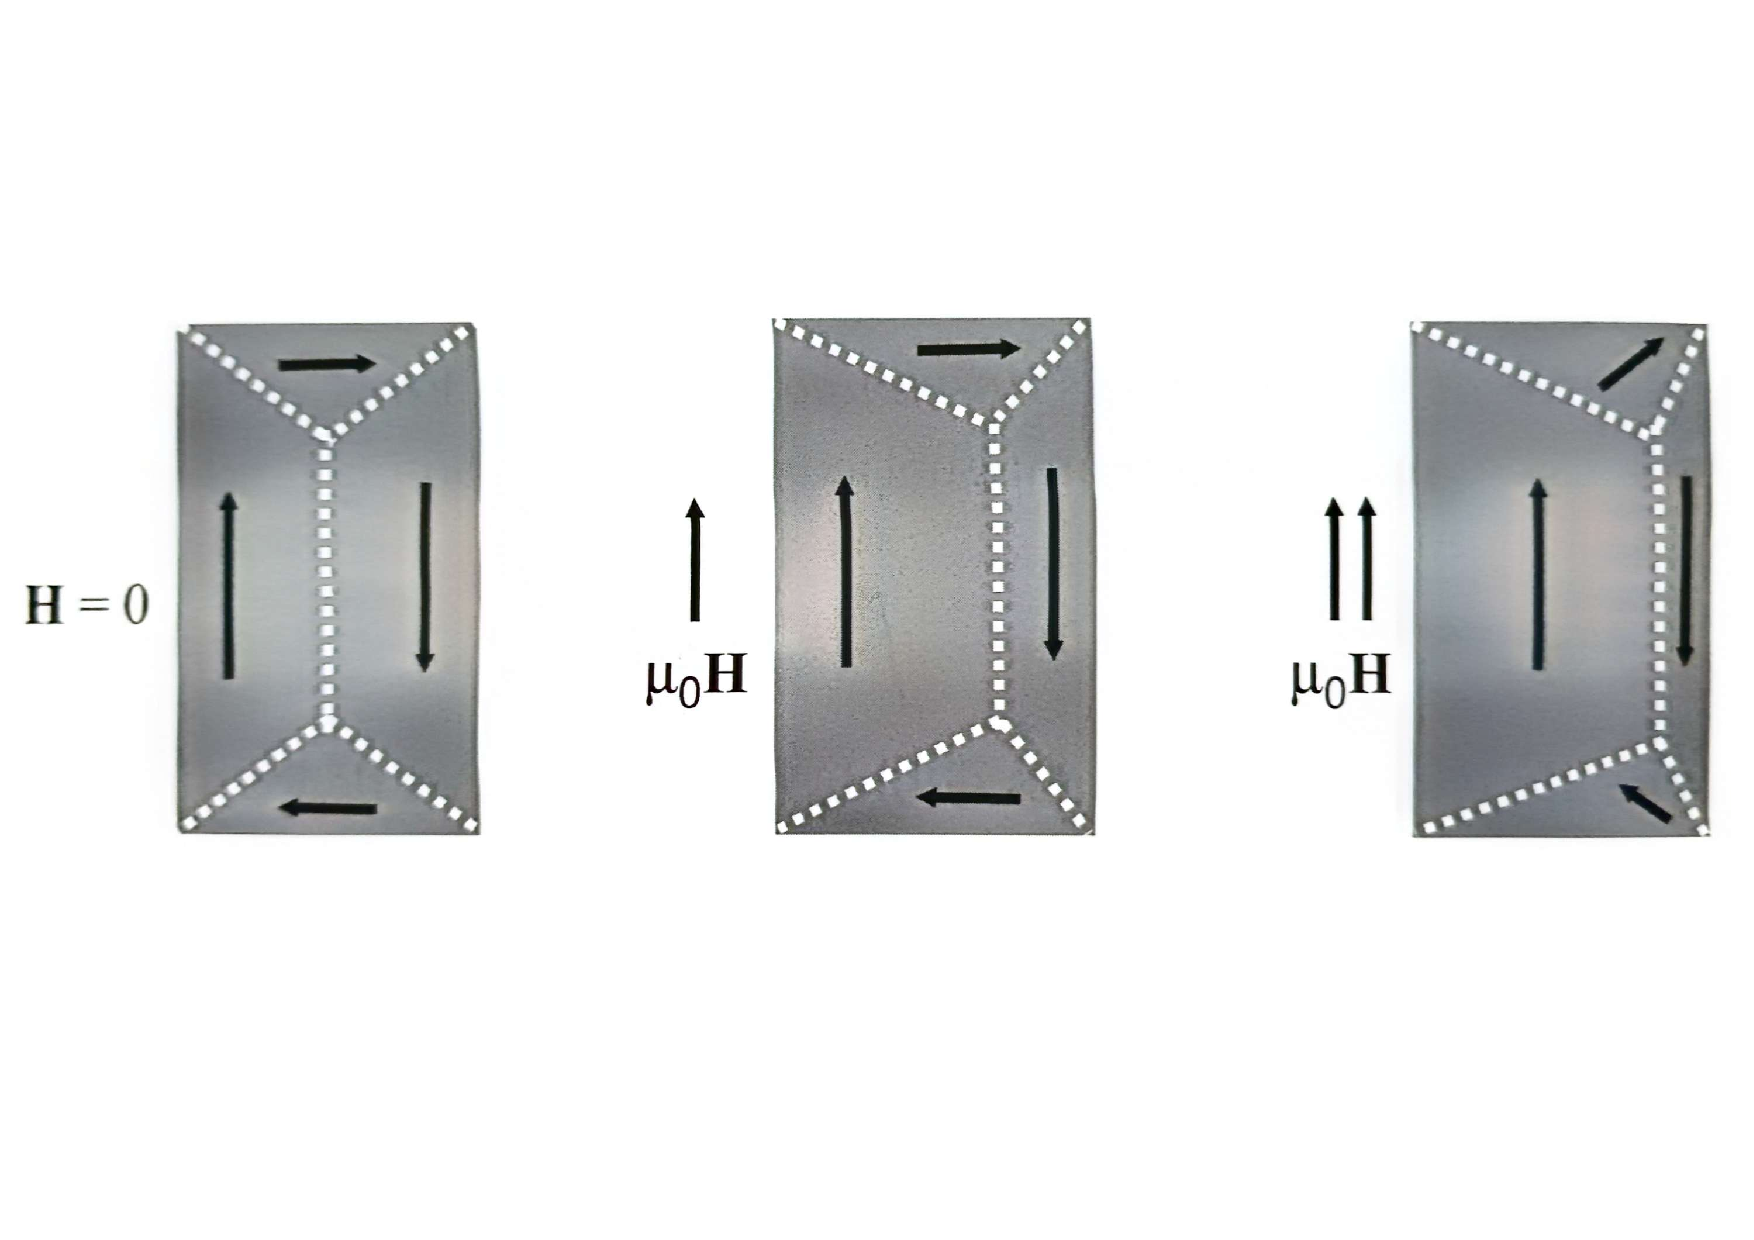
\includegraphics[scale=0.35]{Cuerpo/Ch_10/Fotos libro 8.pdf}
	\caption{Desplazamiento de las fronteras entre dominios debido a una variación del campo magnético aplicado.}
	\label{Fig:10-08}
\end{figure}
\begin{figure}[h!] \centering
	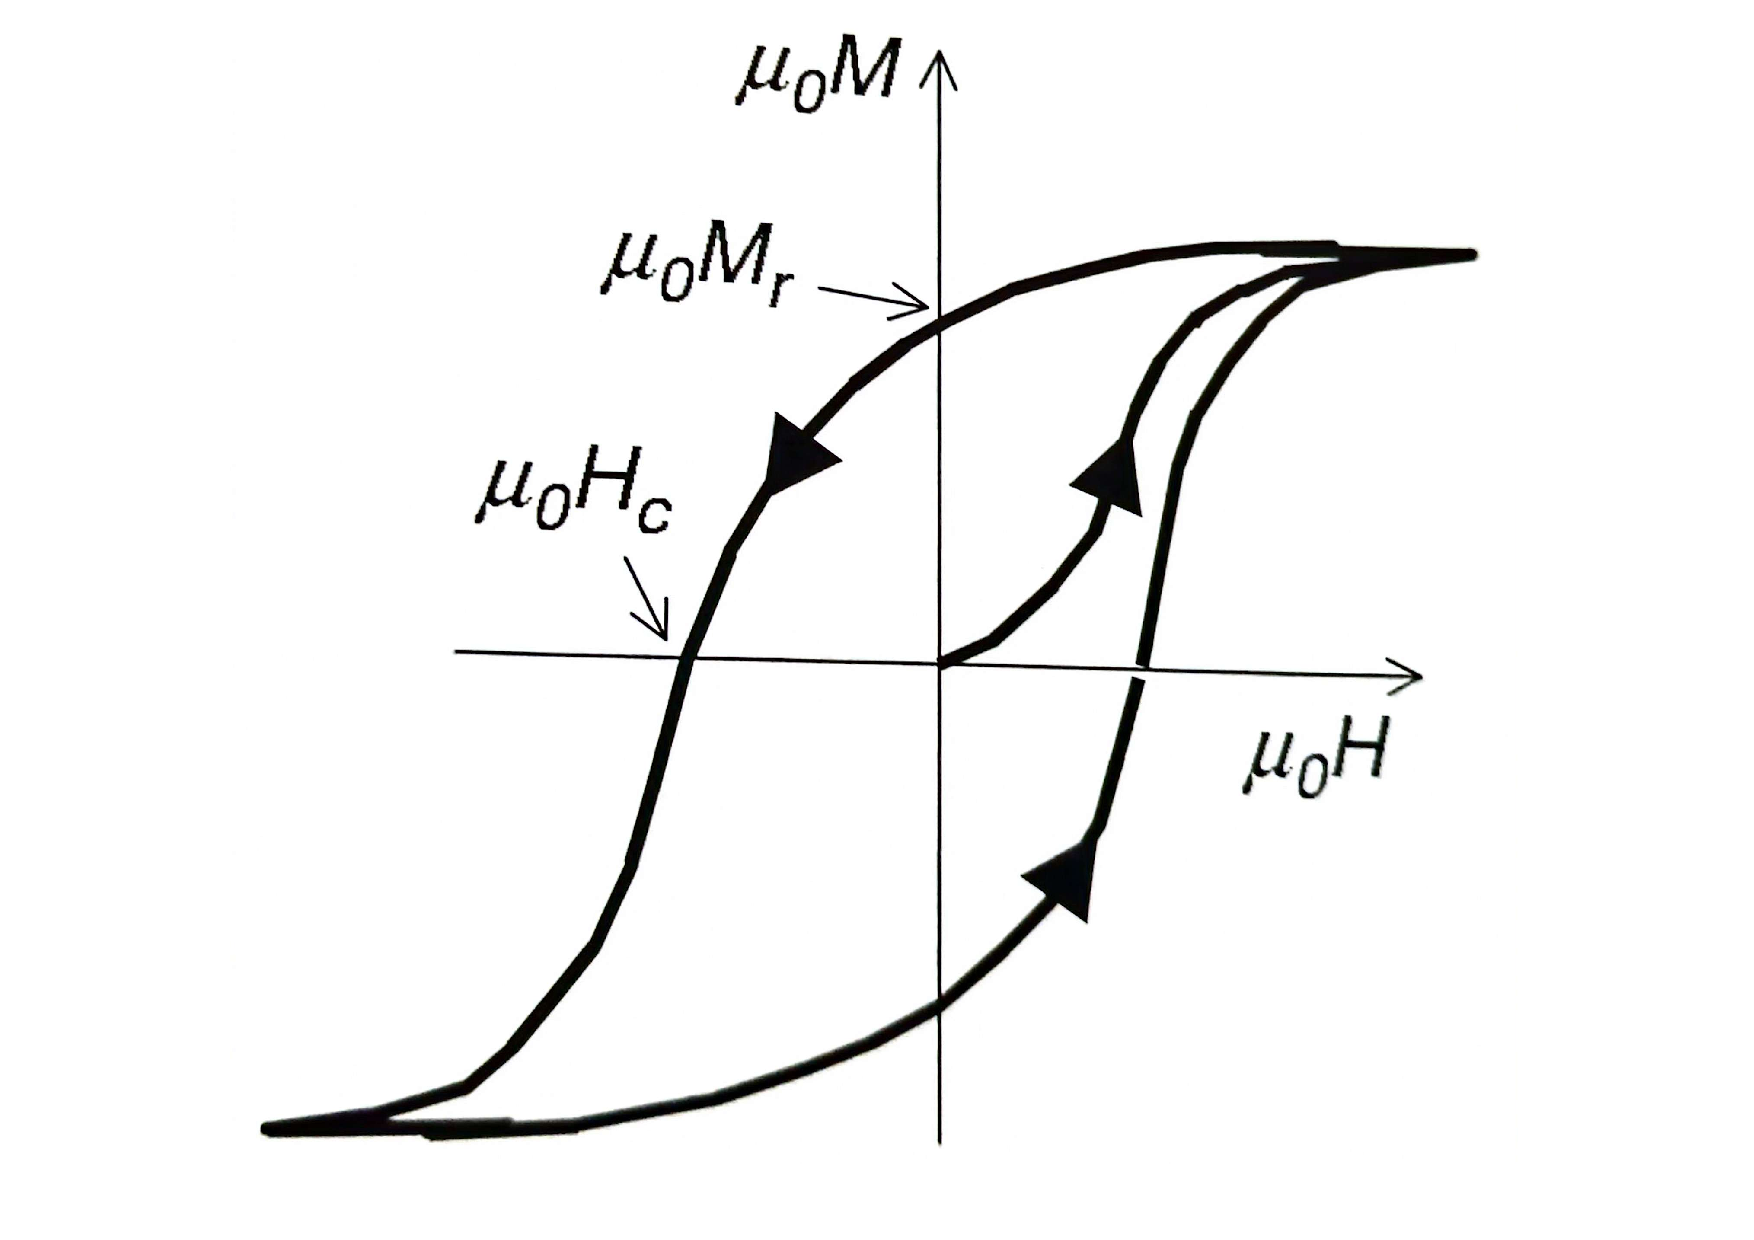
\includegraphics[scale=0.35]{Cuerpo/Ch_10/Fotos libro 9.pdf}
	\caption{Histéresis de la dependencia $M(H)$ debida al anclado de las paredes Bloch en los defectos del material.}
	\label{Fig:10-09}
\end{figure}